% !TEX encoding = UTF-8 Unicode
% !TEX root = ../main.tex
% !TEX spellcheck = en-US

\chapter{Results}
In this chapter, we present the results of this study. 
In this study, we evaluated the design and software quality of the system. This study also addresses all of the research questions. 


%No documentation for pattern usage, but they have a document with coding standard. This includes how to use some patterns. But no docs on where patterns are used, not so big focus on it. 

%Hvor mye er gjenbrukt
%Finne klasser som brukes mye
%Se etter super-klasser
%Memory footprint
%Bruken av C++, gjenbruk kan skape arch drift
%Se etter kode som ikke blir brukt
%Kunne teste ting isolert




\section{Measuring the Software Quality using Metrics}
One way to identify design debt is to measure the software quality using metrics. 



%Metrics for files:
%- Component / Filename
%- Lines of Code
%- Complexity
%- Complexity per function
%- Structure (classes, methods, statements)
%- Functions


% Skal til Research Method



\subsection{Object-Oriented Metrics in Firmus}
In addition to the traditional metrics, we have also gathered data using object-oriented metrics. Traditional software metrics are important for identifying large and complex files, but they alone may not tell us why some classes are large and complex. Object-oriented metrics we have used to measure the quality of the code is mostly based on the work of Chidamber and Kemerer.\cite{chidamber1994metrics}. They have proposed a set of static metrics that are designed to measure the quality of object-oriented software. These metrics are widely known, and their metrics suite is the deepest research in object-oriented metrics investigation and the measurements we have are the following: Weighted Method per Class (WMC), Depth of Inheritance Tree (DIT), Number of Children (NOC), Lack of Cohesion in Methods (LCOM), Response For a Class (RFC), and Coupling between Object Classes (CBO). 


In addition to these metrics, we have chosen to count the number of instance variables and instance methods in each class. A short description of each metric is provided in Section "X". We present their descriptive statistics which includes the minimum, maximum, median, sample mean, and standard deviation values for the whole system. In addition, we present descriptive statistics for each component in the system.

The metric calculation are from several tools i.e., SourceMonitor, Understand, and CCCC. They all provide extensive numbers of software quality metrics.


A description of object-oriented metrics can be found in Chapter 3, Section X. 


\subsection{Object-Oriented Metrics for the whole Project}
 We have decided to exclude the tests from object-oriented metrics analysis. A total of 321 files were analyzed. These files contains 229 classes, and 32068 lines of code. Descriptive statistics such as minimum, maximum, median, sample mean, and standard deviation are presented in this section. Table \ref{tab:oometrics-firmus} presents descriptive statistics for class level metrics for the whole project.

\begin{table}[]
\centering
\caption{OO-metrics for Project Firmus}
\label{tab:oometrics-firmus}
\begin{tabular}{|l|l|l|l|l|l|}
\hline
\textbf{Metric} & \textbf{Min} & \textbf{Max} & \textbf{Median} & \textbf{Sample Mean} & \textbf{Standard Deviation} \\ \hline
LCOM            & 0            & 100          & 55              & 42.205               & 33.042                      \\ \hline
DIT             & 0            & 4            & 1               & 1.061                & 1.062                       \\ \hline
CBO             & 0            & 30           & 5               & 6.079                & 5.179                       \\ \hline
NOC             & 0            & 20           & 0               & 0.454                & 1.850                       \\ \hline
RFC             & 0            & 115          & 10              & 15.777               & 18.677                      \\ \hline
WMC             & 0            & 48           & 7               & 8.616                & 7.167                       \\ \hline
NIM             & 0            & 48           & 7               & 8.376                & 6.983                       \\ \hline
NIV             & 0            & 18           & 1               & 2.223                & 2.811                       \\ \hline
WMC2            & 0            & 325          & 10              & 19.707                 & 31.391                      \\ \hline
\end{tabular}
\end{table}

% TODO: Find X\% of the total classes with high coupling, low cohesion, deep hierarchy. 

\textbf{LCOM}: A class is cohesive if LCOM is low. In this analysis, LCOM is measured in percent. Our data reveals that LCOM value lies between a range from 0 to 100, indicating that there are classes with high and low cohesion. Figure "X" show the frequency distribution of LCOM values. There are 77 classes with LCOM value of 0\%, indicating that these classes has high cohesion. However, 119 classes has a value of LCOM larger than 50\%. Among these, 7 classes have a value of LCOM larger than 90\%, where 2 classes have a LCOM value of 100\%. Classes with low cohesion increases the complexity of the software, and may therefore increase the likelihood of errors during development. In order to improve the class design, it is necessary to split one class to two or more classes to make them more cohesive.

\textbf{DIT and NOC}: DIT value is generally low in the captured statistics. A class with DIT value of 0 is the root in a class hierarchy. Figure "X" shows that 89 classes have a DIT value of 0, and 68 classes have a DIT value of 1. MOreover, DIT value of 2 and 3 indicates higher degree of reuse. In total, we identified 70 classes with DIT value of 2 and 3. The maximum value of DIT captured is set to four. These values show that inheritance is used in most of the classes to an optimal level. However, there may be some possibilities for improvements for classes with DIT value of 0. Moreover, NOC metric measures the number of subclasses of a class. The median value of NOC reveal that half of the classes have NOC value of 0, implying that inheritance may not be used enough. However, the max value of NOC is 20, which may indicate a misuse of subclassing. Classes with high NOC value are difficult to modify, and they usually require more testing because of the effects on changes on all the children. 

\textbf{CBO}: In general, higher values of CBO indicates fault prone classes. Moreover, the reusability of a class will decrease. Our analysis show that 194 classes have a value of CBO less than 10, and 4 classes have a value larger than 20. The maximum value of CBO is 30. This class is an example of a class that is hard to understand, harder to reuse, and more difficult to maintain. 

\textbf{RFC and WMC}: Classes with large RFC tends to be complex and have decreased understandability. Testing classes with large RFC is more complicated. The RFC statistics reveals that majority of the classes have a RFC of less than 20. There are only 22 classes with a value of RFC larger than 30, where 2 of them have a value larger than 100. The maximum value of RFC in this system is 115. In addition, most of the classes have a WMC of less than 7, but there are a few classes with more larger values. Classes with large WMC values may indicate Large Class code smell, and these classes are candidates for inspection and eventually refactoring. 

\textbf{WMC2} By the WMC2 metric, we can observe the complexity of a class by summing complexity of all methods. In general, low values of WMC2 indicates greater polymorphism in a class, while higher higher values of WMC2 indicates more complexity. By examining at Figure "X", we observe that majority of the classes have a value of WMC2 less than 10. More precisely, 123 classes has a value of WMC2 less than 10. Moreover, 5 classes have a value of WMC2 larger than 100. The maximum value of WMC is set to 325.

\textbf{NIM and NIV}: NIM and NIV metric reports the number instance methods and instance variables in a class. Our analysis show that most classes are small. The sample mean of NIV tells us that each class has an average of 2 instance variables. The maximum value of NIV is 18, indicating that there is at least one class that contains 18 instance variables. The sample mean of NIM show us that each class has an average of 8 instance methods. More precisely, there are 170 classes with value of NIM less than 10. The maximum value of NIM is 48, which indicates that there is at least one class contains 48 methods. NIM and NIV metric can help us identify Large Class code smell.


%Good refactoring would be to look at all the classes and see where we could use more abstraction. Reducing redundancy would reduce code size and speed. 

\subsection{Object-Oriented Metrics for the Components}
Descriptive statistics in Table \ref{tab:oometrics-firmus} reveals statistics for class level metrics for the whole project. However, the statistics does not say anything about class level metrics in the different components. Some of the components may have good object-oriented metric values, while other components have bad statistics. In order to identify weak components, we calculated descriptive statistics for each component. 

\subsubsection{Component A}
Component A contains 56 files. Among these files, we identified 40 classes and 6286 lines of code. Figure \ref{fig:algraph} visualizes the frequency distribution of the analyzed object-oriented metrics. Table \ref{tab:oometrics-al} presents common descriptive statistics of the metric distribution.

\begin{table}[]
\centering
\caption{OO-metrics for component A}
\label{tab:oometrics-al}
\begin{tabular}{|l|l|l|l|l|l|}
\hline
\textbf{Metric} & \textbf{Min} & \textbf{Max} & \textbf{Median} & \textbf{Sample Mean} & \textbf{Standard Deviation} \\ \hline
LCOM            & 0            & 94           & 57              & 42.925               & 35.222                      \\ \hline
DIT             & 0            & 4            & 1               & 1.525                & 1.132                       \\ \hline
CBO             & 0            & 29           & 5               & 5.875                & 6.252                       \\ \hline
NOC             & 0            & 8            & 0               & 0.7                  & 1.652                       \\ \hline
RFC             & 2            & 115          & 28.5            & 40.525               & 32.252                      \\ \hline
WMC             & 2            & 44           & 10.5            & 12.675               & 9.339                       \\ \hline
NIM             & 2            & 40           & 10              & 12.3                 & 8.979                       \\ \hline
NIV             & 0            & 12           & 1               & 2.4                  & 2.889                       \\ \hline
WMC2            & 2            & 194          & 17              & 28.9                 & 35.968                      \\ \hline
\end{tabular}
\end{table}

The DIT values indicate that inheritance hierarchies is somehow flat. Classes with flat inheritance hierarchy usually hints that reuse through inheritance is not used. There are approximately eight classes with flat intheritance hierarchy. Rest of the classes inherits for at least one class. The max value captured show that some classes have deep hierarchy. Higher values for DIT indicates higher degree of reuse, but as tradeoff, it may increase complexity of the class. Moreover, the results indicate that most classes only have a few subclasses. Thirty-two classes has no subclasses. However, one class has NOC value of eight. 

The results show that 37.5\% (i.e. 15 classes) of all classes are strongly cohesive, which implies that more than half of the classes show lack of cohesion. By examining Figure \ref{fig:algraph}, we see that two classes has LCOM values larger than 90\%, indicating loose class structures. Furthermore, most classes have small CBO values, indicating that most classes are self-contained. However, the frequency distribution shows that few of the classes are strongly coupled. One class have CBO value of twenty-nine, indicating a possible fault-prone class which affects its reusability and maintainability. This particular class has LCOM value of 62, WMC2 value of 95, and RFC value of 25.

The results show that each class have at least two methods. More than half of the classes have low RFC values, which indicates greater polymorphism. However, there are few classes in this component that has more high RFC. The maximum RFC is 115, and classes with high RFC are usually difficult to maintain and test. However, the class with a RFC value of 115 has 

The values of WMC2 ranges from 2 to 194. The median value indicate that half of the classes have a cyclomatic complexity of 17 or less. However, the sample mean is revealed to be larger than the median value. This implies that there are few classes with large values of WMC2, which is evident by inspecting the standard deviation.

Classes with large number of instance variables are few. More than half of the classes has one instance variable or less. The largest number of instance variables is 12, revealing that software system does not apply information hiding principle appropriately for this class. Furthermore, each class is revealed to have two instance methods. Approximately 50\% of the classes have 10 instance methods or less. This means that rest of the classes have more than 10 instance methods, which indicates that classes may provide several services to other classes. The maximum value of NIM captured is 40. There are two classes with NIM value of 40, one having a WMC2 value of 194 and the other having a WMC2 value of 72. 


AL: LogicsEngine
Autrologic: LogicsUnitDetectionZone
Autrologic: Logicsunit
AL: LogicsUnitFad (kasnkje)
BLC: AclibTranslator



\begin{landscape}
\setlength\LTleft{-.5in}
	\begin{figure}
	\label{fig:algraph}
	\caption{Frequency distribution of OO-metrics in Component A}
	\centering
	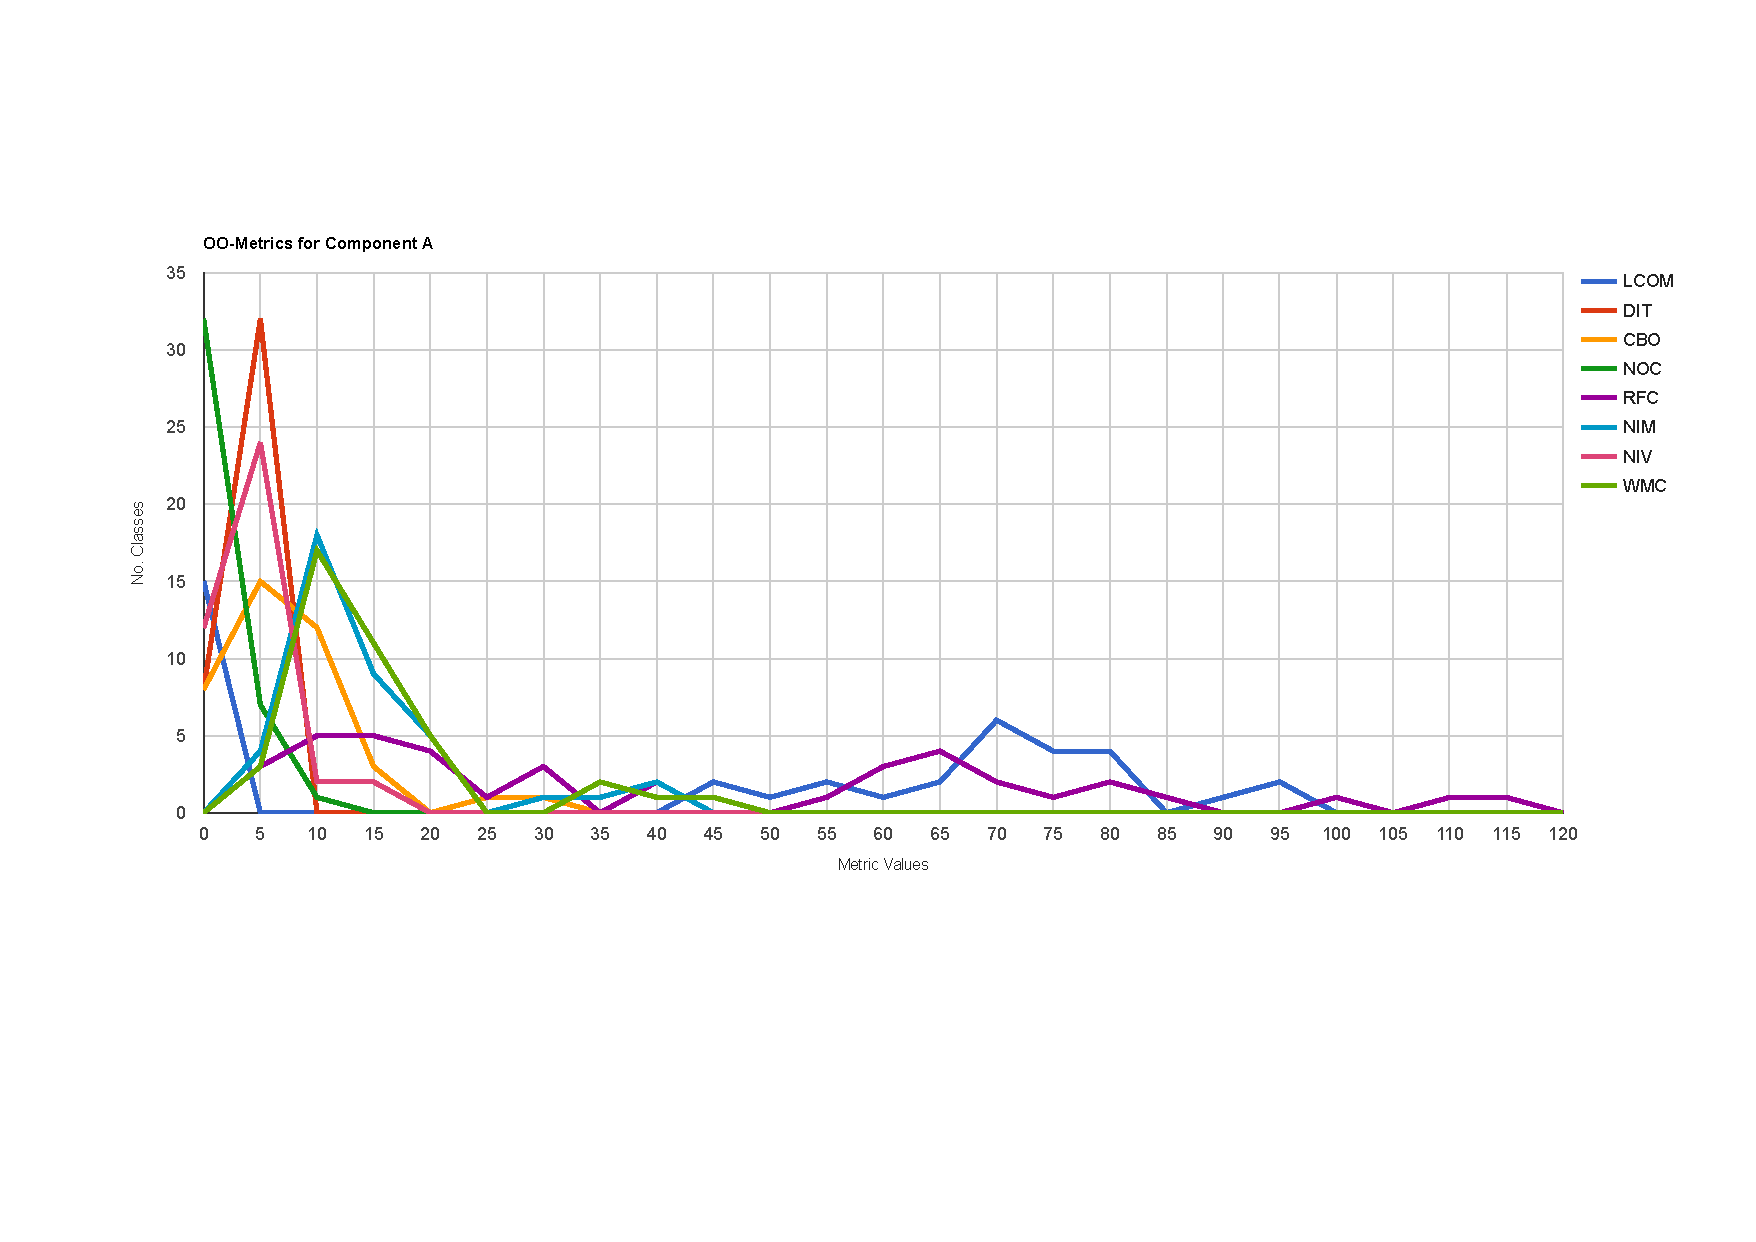
\includegraphics[width=\textwidth]{images/al.pdf}
	\end{figure}
\end{landscape}

% 2 large code smell




\subsubsection{Component B}
We identified 23 classes in Component B. These classes are spread across 42 files, which in total contains 3905 lines of code. Figure \ref{fig:blcgraph} presents a frequency chart of the object-oriented metric results for Component B. Table \ref{tab:oometrics-blc} presents descriptive statistics of the analyzed metrics.

The values of LCOM in Component B range from 22 to 90 percent, indicating none of the classes are cohesive. There are only two classes with LCOM values below 50, both having low values in terms of cyclomatic, method count, coupled objects, and instance variables. Moreover, the WMC2 values ranges from 3 to 325. We decided to examine the class with a WMC2 value of 325. This class has a LCOM value of 74, and a CBO value of 10. Its RFC value is 44, while NIM and WMC is both 36. This class has no subclasses, but it does inherits methods and variables from one superclass. In terms of cyclomatic complexity, we believe that this class is the most complex class in this system. Moreover, there are 8 classes in this component with a LCOM value of 66. By examining the metrics of these classes, we did notice that 4 of these classes has identical DIT, CBO, RFC, NIM, NIV, WMC, and WMC2 values. Manual inspection of the classes did not reveal any duplicated code. However, in terms of refactoring, we do think that all these classes need the same effort.

% to mulige store klasser.


\begin{table}[]
\centering
\caption{OO-metrics for Component B}
\label{tab:oometrics-blc}
\begin{tabular}{|l|l|l|l|l|l|}
\hline
\textbf{Metric} & \textbf{Min} & \textbf{Max} & \textbf{Median} & \textbf{Sample Mean} & \textbf{Standard Deviation} \\ \hline
LCOM            & 22           & 90          & 66              & 63.479               & 15.753                    \\ \hline
DIT             & 0           & 1           & 1             & 0.609              & 0.499                       \\ \hline
CBO             & 1          & 22           & 5              & 6.348                & 5.077                       \\ \hline
NOC             & 0            & 1           & 0               & 0.087                & 0.288                       \\ \hline
RFC             & 6            & 44          & 9              & 13.956               & 11.055                      \\ \hline
WMC             & 6            & 40           & 9              & 13.261                & 9.992                       \\ \hline
NIM             & 6           & 40           & 9               & 13.261                & 9.992                       \\ \hline
NIV             & 1            & 10           & 2               & 3                & 2.504                       \\ \hline
WMC2            & 3            & 325          & 20              & 37.696               & 66.466                      \\ \hline
\end{tabular}
\end{table}


\begin{landscape}
\setlength\LTleft{-.5in}
	\begin{figure}
	\label{fig:blcgraph}
	\caption{Frequency distribution of OO-metrics in Component B}
	\centering
	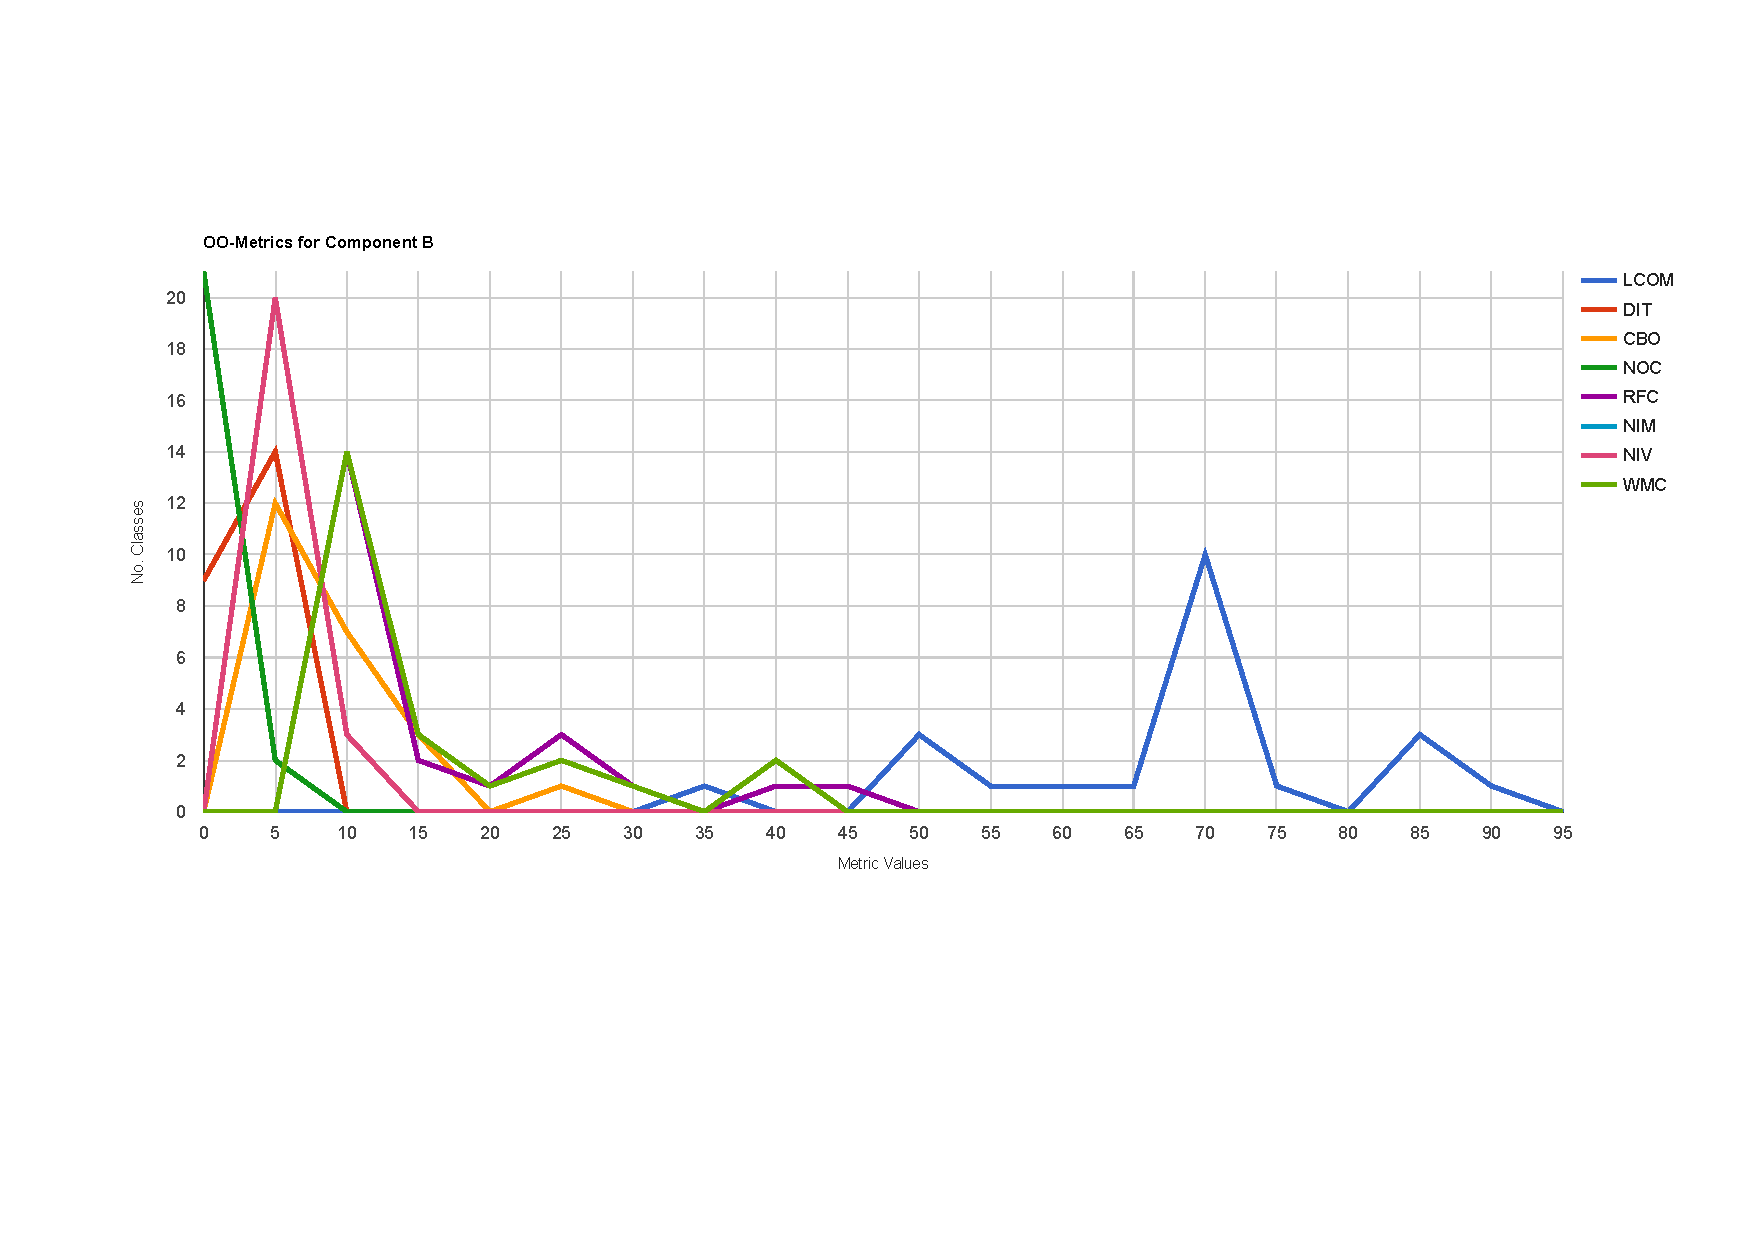
\includegraphics[width=\textwidth]{images/blc.pdf}
	\end{figure}
\end{landscape}



\subsubsection{Component C}
Our analysis shows that component C contains 30 files, 20 classes, and 4763 lines of code. We present the descriptive statistics for component C in Table \ref{tab:oometrics-config}, and the frequency distribution of the metrics in Figure \ref{fig:confgraph}.

LCOM value of Component C ranges from 0 to 99. The median shows that more than half of the classes have LCOM value of 60 or more, indicating possibilities for design improvements by splitting up the classes. DIT and NOC metric values is very low, implying that inheritance may not be used. Moreover, CBO values ranges from 1 to 18. Each class has a CBO value of 5 in average. The results show that there is one class with CBO value of 18. This class prevents reuse due to its modular design. Strong coupling complicates a system since a class is harder to understand and modify. WMC2 metric values ranges from 2 to 106. The median value implies that half of the classes has a complexity value of 9, implying that complexity is well managed for those classes. However, the maximum value tells us that there is one complex class in this component. This particular class has a LCOM value of 63, and is coupled to 18 other objects, hence being the class with CBO value of 18. RFC, WMC, and NIM values of this class is 26, all maximum values that we analyzed. All these values are an indication of a possible fault-prone and complex class. In addition, this class may be affected by the Large Class code smell.

% 1 large class code smell, mulig 2. 



\begin{table}[]
\centering
\caption{OO-metrics for Component C}
\label{tab:oometrics-config}
\begin{tabular}{|l|l|l|l|l|l|}
\hline
\textbf{Metric} & \textbf{Min} & \textbf{Max} & \textbf{Median} & \textbf{Sample Mean} & \textbf{Standard Deviation} \\ \hline
LCOM            & 0            & 99           & 61              & 55.7                 & 23.58                       \\ \hline
DIT             & 0            & 1            & 0               & 0.1                  & 0.308                       \\ \hline
CBO             & 1            & 18           & 4               & 5.55                 & 4.662                       \\ \hline
NOC             & 0            & 0            & 0               & 0                    & 0                           \\ \hline
RFC             & 3            & 26           & 8.5             & 10.3                 & 5.741                       \\ \hline
WMC             & 3            & 26           & 8.5             & 10.3                 & 5.741                       \\ \hline
NIM             & 3            & 26           & 8.5             & 9.85                 & 5.153                       \\ \hline
NIV             & 0            & 9            & 2               & 3.15                 & 3.013                       \\ \hline
WMC2            & 2            & 106          & 9              & 23.25                 & 27.733                      \\ \hline
\end{tabular}
\end{table}



\begin{landscape}
\setlength\LTleft{-.5in}
	\begin{figure}
	\label{fig:confgraph}
	\centering
	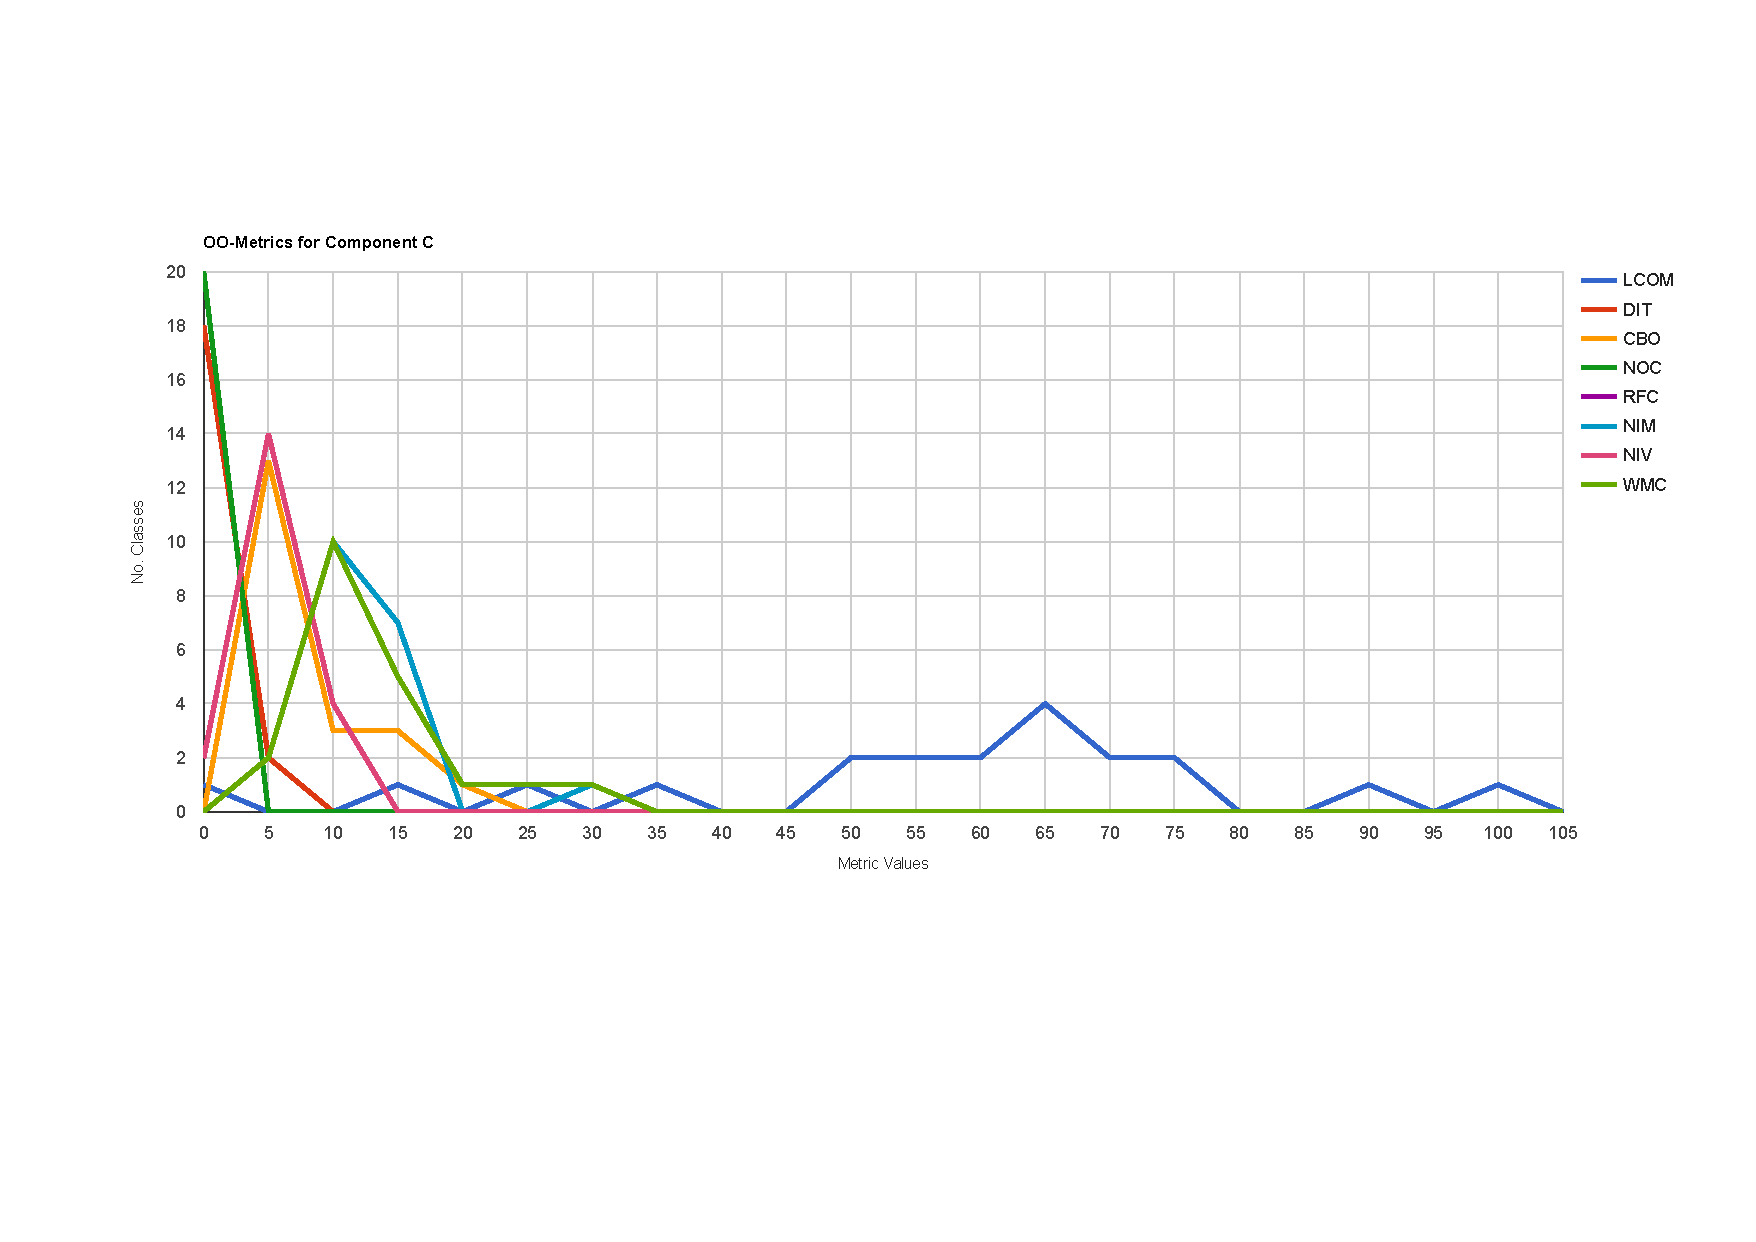
\includegraphics[width=\textwidth]{images/conf.pdf}
	\end{figure}
\end{landscape}


\subsubsection{Component D}
Our analysis show that Component D consists of 13 files and 1647 lines of code. Among these files, we identified only one class. This class has LCOM value of 68, which tells that the class is not very cohesive. Furthermore, our result show a DIT value of 1, an NOC value of 0, indicating that this class only inherits from a superclass. The CBO value is set to 7, implying that this class is coupled to 7 objects. The values of RFC, WMC, and NIM have a value of 8. Moreover, the class however has only 1 instance variable. The sum of complexity in this class is 17.



\subsubsection{Component En}
Similar to Component D, our analysis identified only one class among 3 files and 367 lines of code in Component En. The metrics are very similar to Component D metrics. The class has a LCOM value of 62, indicating low cohesion in some of the methods. However, compared to Component D, this class is only coupled to one object. The sum of complexity of methods in this class is 15.


\subsubsection{Component Ex}
Our analysis found 48 files in Component Ex. These files consist of 4089 lines of code, and among these, we identified 86 classes. 38\% of the number of classes in we identified in this system is located in this component. Table \ref{tab:oometrics-ex} present the descriptive statistics for Component Ex, while Figure \ref{fig:exgraph} present the frequency distribution of the measured metrics. 

The values of LCOM ranges from 0 to 100, indicating that there are classes with low and high cohesion. The median value of LCOM is 0, implying that half of the classes in this component has high cohesion.  Even though half of the classes has high cohesion, there are still many classes with low cohesion. Our results show that there are 22 classes with LCOM value larger than 50, where 6 classes has LCOM value of 80 or more. There are only 2 classes with LCOM value of 100. Moreover, the average cyclomatic complexity of the classes has a value of 8.7, while the median has a value of 7. These values implies that most classes may have more polymorphism and less complexity. Figure \ref{fig:exgraph} shows us that there are only one 8 classes with value of WMC2 larger than 20, where the maximum value is 41. These values indicates that the complexity is well managed to this point. By examining the CBO values, we observe that only 7 classes are self-contained. The rest of the classes are coupled to other objects. The majority of the classes has a CBO value of 5 or less. There is only one class with CBO value of 16, indicating that this class may be difficult to understand and maintain. The result show a RFC range from 0 to 28, with more than 50\% of the classes having RFC value of 10 or less.

\begin{table}[]
\centering
\caption{OO-metrics for Component Ex}
\label{tab:oometrics-ex}
\begin{tabular}{|l|l|l|l|l|l|}
\hline
\textbf{Metric} & \textbf{Min} & \textbf{Max} & \textbf{Median} & \textbf{Sample Mean} & \textbf{Standard Deviation} \\ \hline
LCOM            & 0           & 100          & 0               & 25.988               & 32.905                      \\ \hline
DIT             & 0            & 3            & 2               & 1.581                & 1.121                       \\ \hline
CBO             & 0            & 16           & 4               & 4.919                & 4.018                       \\ \hline
NOC             & 0            & 20           & 0               & 0.744                & 2.736                       \\ \hline
RFC             & 0            & 28           & 8               & 10.279               & 6.030                       \\ \hline
WMC             & 0            & 22           & 3.5             & 5.07                 & 3.928                       \\ \hline
NIM             & 0            & 22           & 3               & 4.907                & 3.846                       \\ \hline
NIV             & 0            & 10           & 0               & 1.209                & 2.098                       \\ \hline
WMC2            & 0            & 41          & 7              & 8.744                 & 8.117                      \\ \hline
\end{tabular}
\end{table}


\begin{landscape}
\setlength\LTleft{-.5in}
	\begin{figure}
	\label{fig:exgraph}
	\caption{Coming}
	\centering
	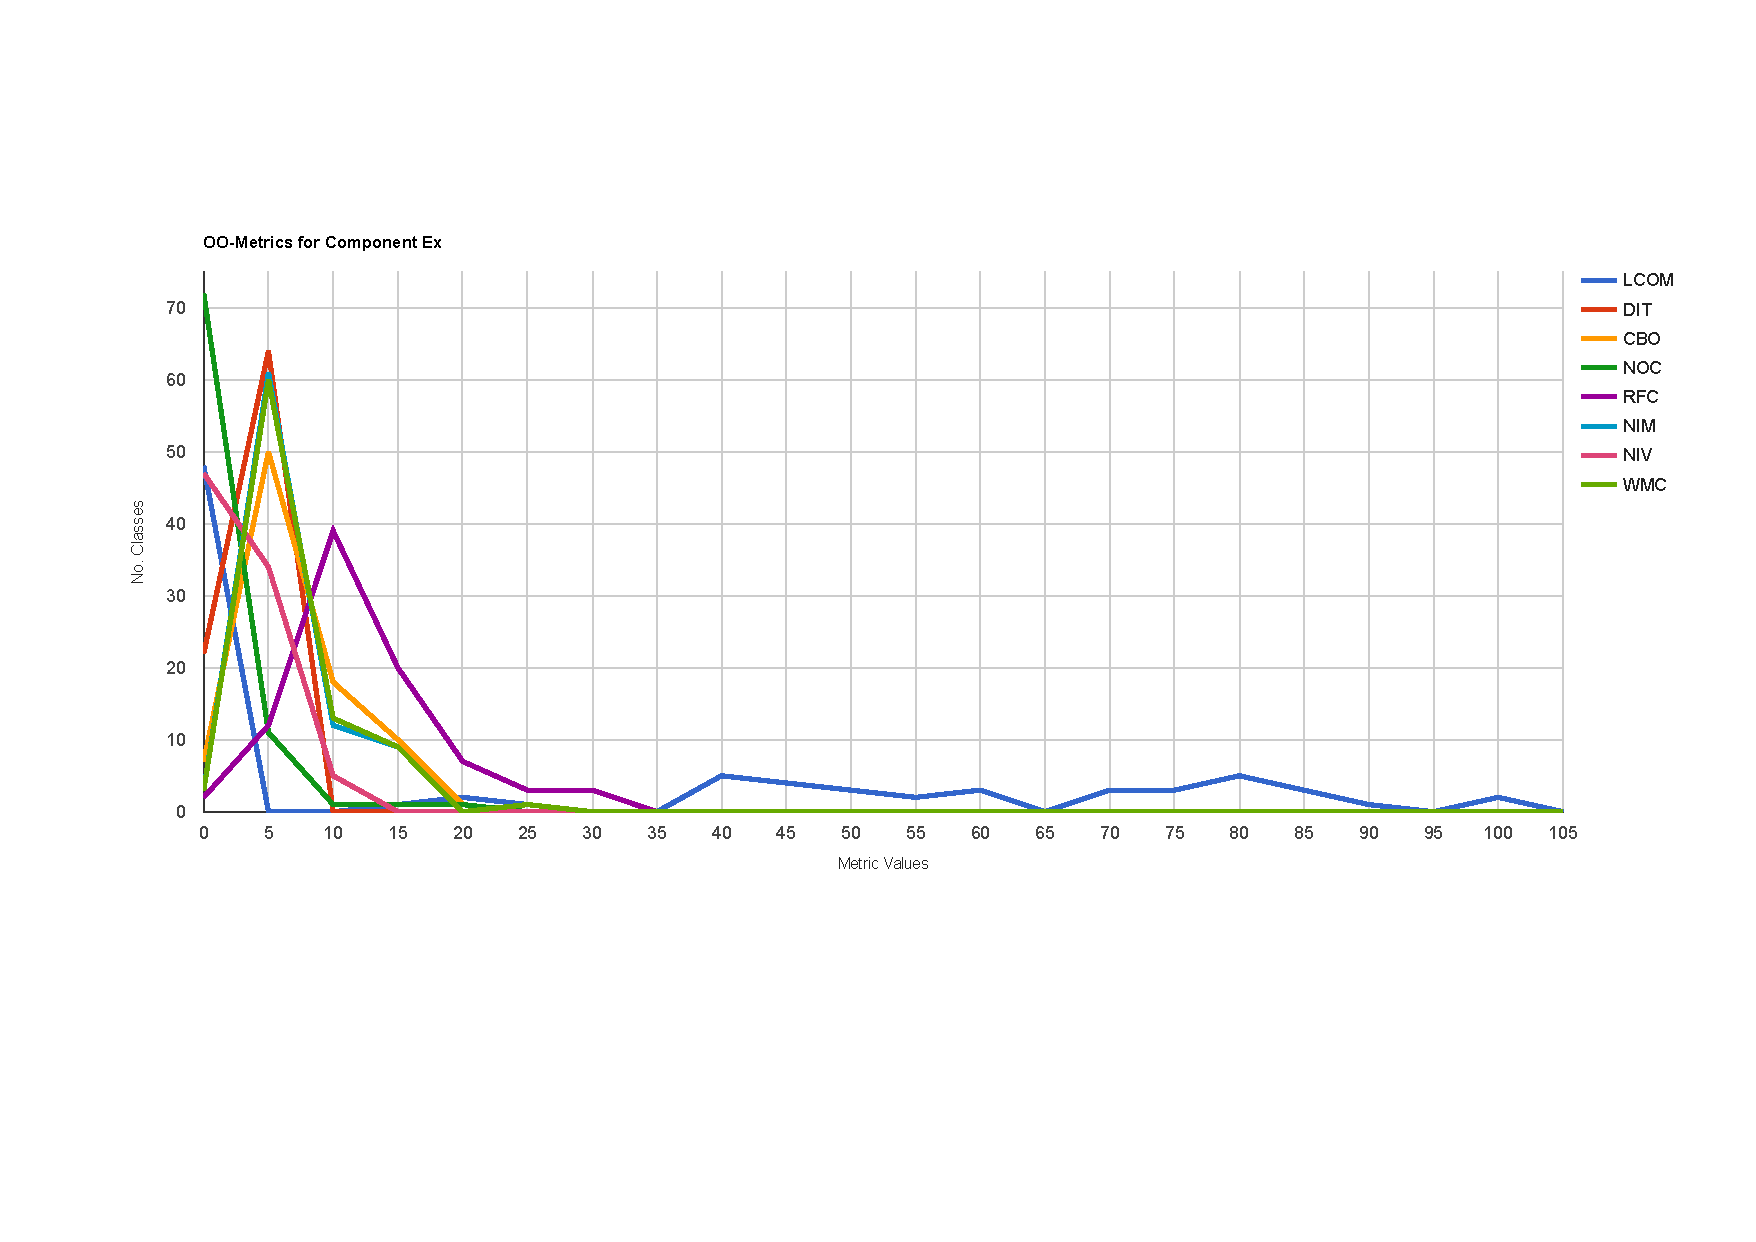
\includegraphics[width=\textwidth]{images/ex.pdf}
	\end{figure}
\end{landscape}


% GOd class detection: High WMC, low cohesion, number of attributes bigger than 20




\subsubsection{Component G}
Component G consists of 59 files. These files includes 3701 lines of code and 32 classes. Descriptive statistics for Component G is summarized in Table \ref{tab:oometrics-guri}, and its frequency distribution of the metrics can be seen in Figure \ref{fig:gurigraph}. 

Overall, the statistics are indicating that there are some accumulated design debt in this component. The values of LCOM ranges from 0 to 94, where 8 classes has a LCOM value of 0. However, values of LCOM for rest of the classes are larger than 50. Moreover, the statistics show that 18 classes have a DIT value of larger than 0, indicating a higher degree of reuse. There are only 5 classes with subclasses in this component. WMC2 values in this component ranges from 1 to 123, where only class has a value of WMC2 larger than 100. We decided to examine the class with WMC2 value of 123. The results show that this class has a LCOM value of 92, CBO value of 22, RFC value of 30, NIM value of 9, NIV value of 18, and WMC value of 30. These values say that this class is probably influenced by the Large Class code smell, and is a candidate for inspection and refactoring.



\begin{table}[]
\centering
\caption{Component G}
\label{tab:oometrics-guri}
\begin{tabular}{|l|l|l|l|l|l|}
\hline
\textbf{Metric} & \textbf{Min} & \textbf{Max} & \textbf{Median} & \textbf{Sample Mean} & \textbf{Standard Deviation} \\ \hline
LCOM            & 0            & 94           & 60              & 50.25                & 31.236                      \\ \hline
DIT             & 0            & 2            & 1               & 0.625                & 0.609                       \\ \hline
CBO             & 0            & 22           & 5.5             & 6.187                & 4.987                       \\ \hline
NOC             & 0            & 2            & 0               & 0.25                 & 0.622                       \\ \hline
RFC             & 2            & 30           & 9               & 10.187               & 6.382                       \\ \hline
WMC             & 2            & 30           & 7.5             & 8.594                & 5.405                       \\ \hline
NIM             & 0            & 29           & 7               & 8.437                & 5.459                       \\ \hline
NIV             & 0            & 18           & 2               & 3.062                & 3.926                       \\ \hline
WMC2            & 1            & 123          & 12              & 19.437                 & 24.794                      \\ \hline
\end{tabular}
\end{table}

\begin{landscape}
\setlength\LTleft{-.5in}
	\begin{figure}
	\label{fig:gurigraph}
	\caption{Coming}
	\centering
	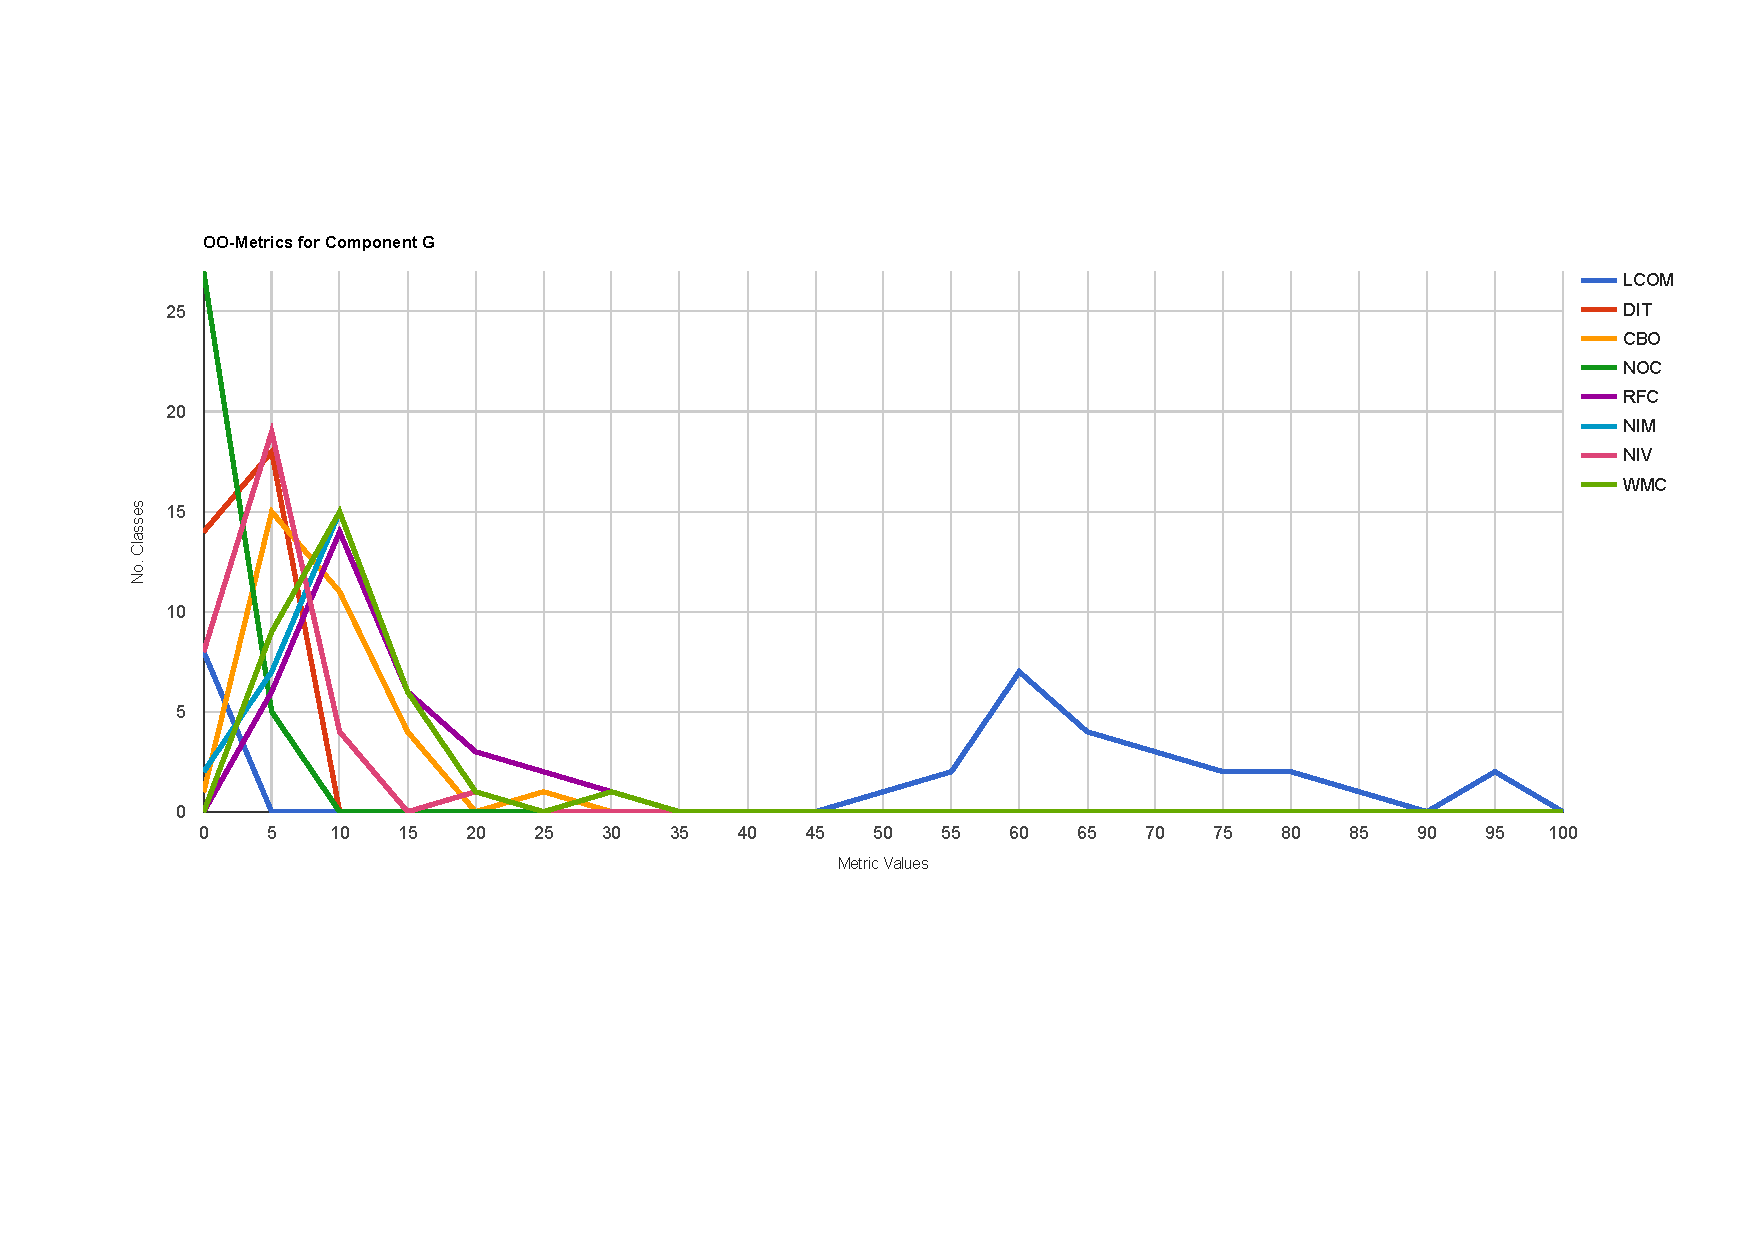
\includegraphics[width=\textwidth]{images/guri.pdf}
	\end{figure}
\end{landscape}





\subsubsection{Component L}
Component L consist of 16 files, 849 lines of code. Among these, we identified 7 classes. Figure \ref{fig:loggraph} presents the frequency distribution of the metrics, while Table \ref{tab:oometrics-log} presents the descriptive statistics for this component. The values of LCOM range from 0 to 80. There are only 2 classes with LCOM value at 0. However, rest of the classes are showing lack of cohesion. These classes are candidates for inspection, and should eventually be split up into multiple classes. Moreover, 4 classes have a DIT value of 1. WMC2 values ranges from 4 to 42. There are only 2 classes with WMC2 values larger than 30.

\begin{table}[]
\centering
\caption{OO-metrics for Component L}
\label{tab:oometrics-log}
\begin{tabular}{|l|l|l|l|l|l|}
\hline
\textbf{Metric} & \textbf{Min} & \textbf{Max} & \textbf{Median} & \textbf{Sample Mean} & \textbf{Standard Deviation} \\ \hline
LCOM            & 0            & 80           & 58              & 50.857               & 35.130                      \\ \hline
DIT             & 0            & 1            & 1               & 0.571                & 0.534                       \\ \hline
CBO             & 1            & 13           & 4               & 5.571                & 4.197                       \\ \hline
NOC             & 0            & 0            & 0               & 0                    & 0                           \\ \hline
RFC             & 5            & 12           & 9               & 8.571                & 2.936                       \\ \hline
WMC             & 5            & 12           & 9               & 8.571                & 2.936                       \\ \hline
NIM             & 3            & 12           & 7               & 8.286                & 3.402                       \\ \hline
NIV             & 0            & 5            & 1               & 1.571                & 2.070                       \\ \hline
WMC2            & 4            & 42          & 11              & 19.571                 & 14.524                      \\ \hline
\end{tabular}
\end{table}



\begin{landscape}
\setlength\LTleft{-.5in}
	\begin{figure}
	\label{fig:loggraph}
	\caption{Coming}
	\centering
	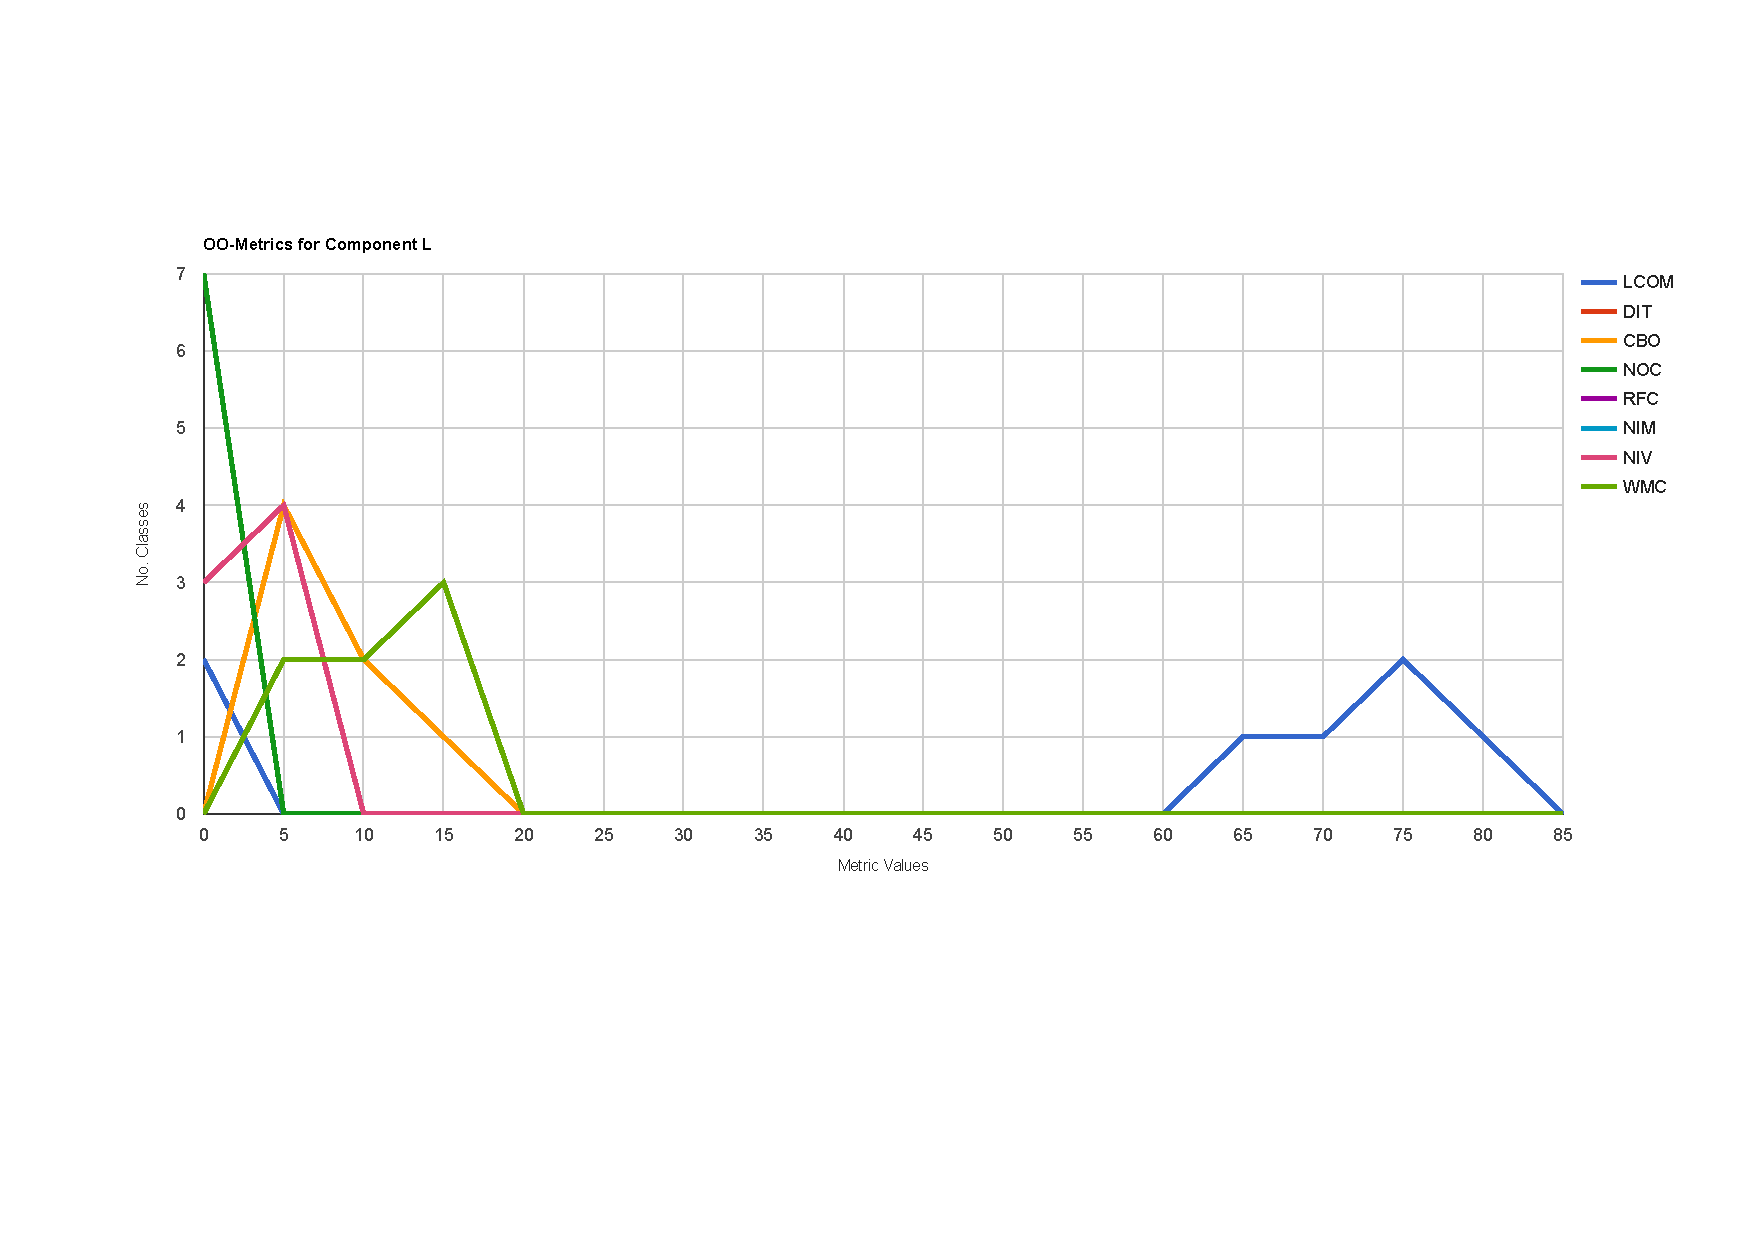
\includegraphics[width=\textwidth]{images/log.pdf}
	\end{figure}
\end{landscape}







\subsubsection{Component N}
Component N consists of 17 files. In total, there are 1839 lines of code spread across these files. We identified 8 classes in this component. Descriptive statistics for Component N are presented in Table \ref{tab:oometrics-netw}, while the frequency distribution of the metrics are presented in Figure \ref{fig:netgraph}.

LCOM metric value ranges from 0 to 79. The median value show that more than half of the classes has LCOM value of 70 or more, indicating that this component should be split into more classes to increase the cohesion of each class. By taking a closer look at Figure \ref{fig:netgraph}, we identify two classes with LCOM values interval from 75 to 80. More precisely, one class has LCOM value of 78 while the other class has LCOM value of 79. We decided to examine the class with LCOM value of 79, and identified that this class has WMC2 value of 125, RFC value of 32, CBO value of 17, WMC value of 23 and NIM value of 21. These values tells us that this class may be affected by Large Class and God Class code smell.


\begin{table}[]
\centering
\caption{OO-metrics for Component N}
\label{tab:oometrics-netw}
\begin{tabular}{|l|l|l|l|l|l|}
\hline
\textbf{Metric} & \textbf{Min} & \textbf{Max} & \textbf{Median} & \textbf{Sample Mean} & \textbf{Standard Deviation} \\ \hline
LCOM            & 0            & 79           & 70.5            & 54.5                 & 33.899                      \\ \hline
DIT             & 0            & 1            & 0               & 0.25                 & 0.463                       \\ \hline
CBO             & 3            & 17           & 10.5            & 10                   & 4.140                       \\ \hline
NOC             & 0            & 1            & 0               & 0.125                & 0.353                       \\ \hline
RFC             & 6            & 32           & 9               & 11.625               & 8.568                       \\ \hline
WMC             & 6            & 23           & 9               & 10.5                 & 5.580                       \\ \hline
NIM             & 6            & 21           & 8.5             & 9.75                 & 5.036                       \\ \hline
NIV             & 0            & 8            & 5.5             & 4.375                & 3.068                       \\ \hline
WMC2            & 4            & 125          & 32              & 40.375                 & 36.707                      \\ \hline
\end{tabular}
\end{table}


\begin{landscape}
\setlength\LTleft{-.5in}
	\begin{figure}
	\label{fig:netgraph}
	\caption{Coming}
	\centering
	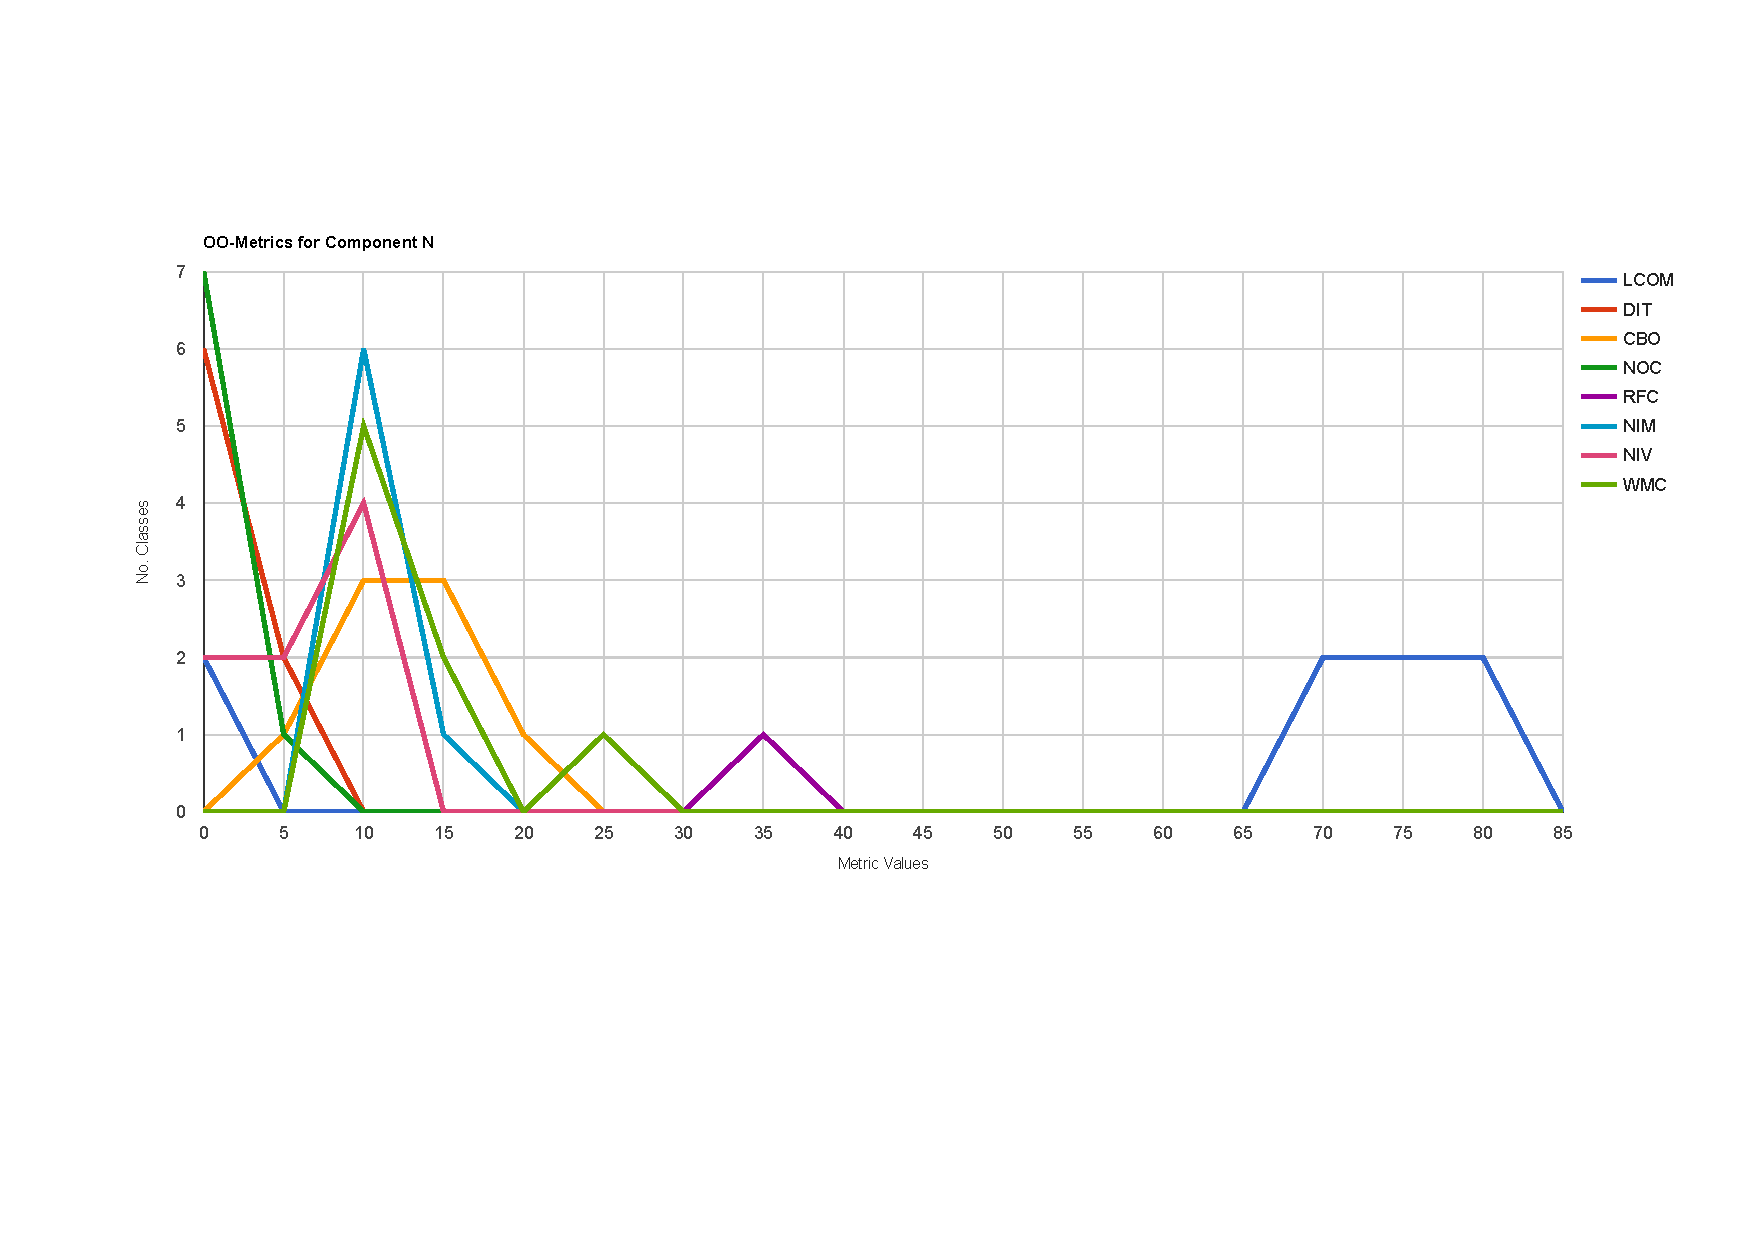
\includegraphics[width=\textwidth]{images/network.pdf}
	\end{figure}
\end{landscape}



\subsubsection{Component P}
Descriptive statistics calculated for Component P are presented in Table \ref{tab:oometrics-proc}. The frequency distribution of the metrics are presented in Figure \ref{fig:procgraph}. We identified 12 files in Component P, consisting of 12 files, 722 lines of code, and 8 classes.

In case of measurement for cohesion, LCOM values in Component P lies between a range from zero percent to eight-one percent. A median value shows the level of cohesiveness in the system. In this context, median value show that more than half of the classes have large LCOM values, implying that these classes are improperly designed and should be split up to make them cohesive. By examining the component, we identified three classes with values of LCOM larger than 70. The DIT results range from 0 to 1, implying that most classes have flat inheritance hierarchies. There are only 2 classes having a DIT value of 1. Despite the fact that 6 of the classes have DIT metric of 0, they alone may not tell us if classes are part of an inheritance tree or if they are root classes. By examining the NOC results, we see that only one class has a NOC value of 1. Six classes have both NOC and DIT values of zero, indicating that they are not part of an inheritance hierarchy. CBO values lies between a range from zero to twelve, with a mean and median of 5.5. In addition, WMC2 values lies between a range from 1 to 47, where two classes has WMC2 values larger than 30. In addition, we were able to identify a complex class, possible a God Class code smell. This class has a LCOM value of 77, WMC2 value of 47, and DIT value of 1. Moreover, the class has 13 methods, and RFC value of 14.


\begin{table}[]
\centering
\caption{OO-metrics for Component P}
\label{tab:oometrics-proc}
\begin{tabular}{|l|l|l|l|l|l|}
\hline
\textbf{Metric} & \textbf{Min} & \textbf{Max} & \textbf{Median} & \textbf{Sample Mean} & \textbf{Standard Deviation} \\ \hline
LCOM            & 0            & 81           & 65              & 58.25                & 26.611                      \\ \hline
DIT             & 0            & 1            & 0               & 0.25                 & 0.463                       \\ \hline
CBO             & 0            & 12           & 5.5             & 5.5                  & 3.964                       \\ \hline
NOC             & 0            & 1            & 0               & 0.125                & 0.353                       \\ \hline
RFC             & 2            & 14           & 6.5             & 7.5                  & 3.625                       \\ \hline
WMC             & 2            & 14           & 6.5             & 7.25                 & 3.412                       \\ \hline
NIM             & 2            & 13           & 6.5             & 7                    & 3.117                       \\ \hline
NIV             & 0            & 6            & 3.5             & 3.125                & 2.031                       \\ \hline
WMC2            & 1            & 47           & 8               & 15.75                & 15.809                      \\ \hline
\end{tabular}
\end{table}



\begin{landscape}
\setlength\LTleft{-.5in}
	\begin{figure}
	\label{fig:procgraph}
	\caption{Coming}
	\centering
	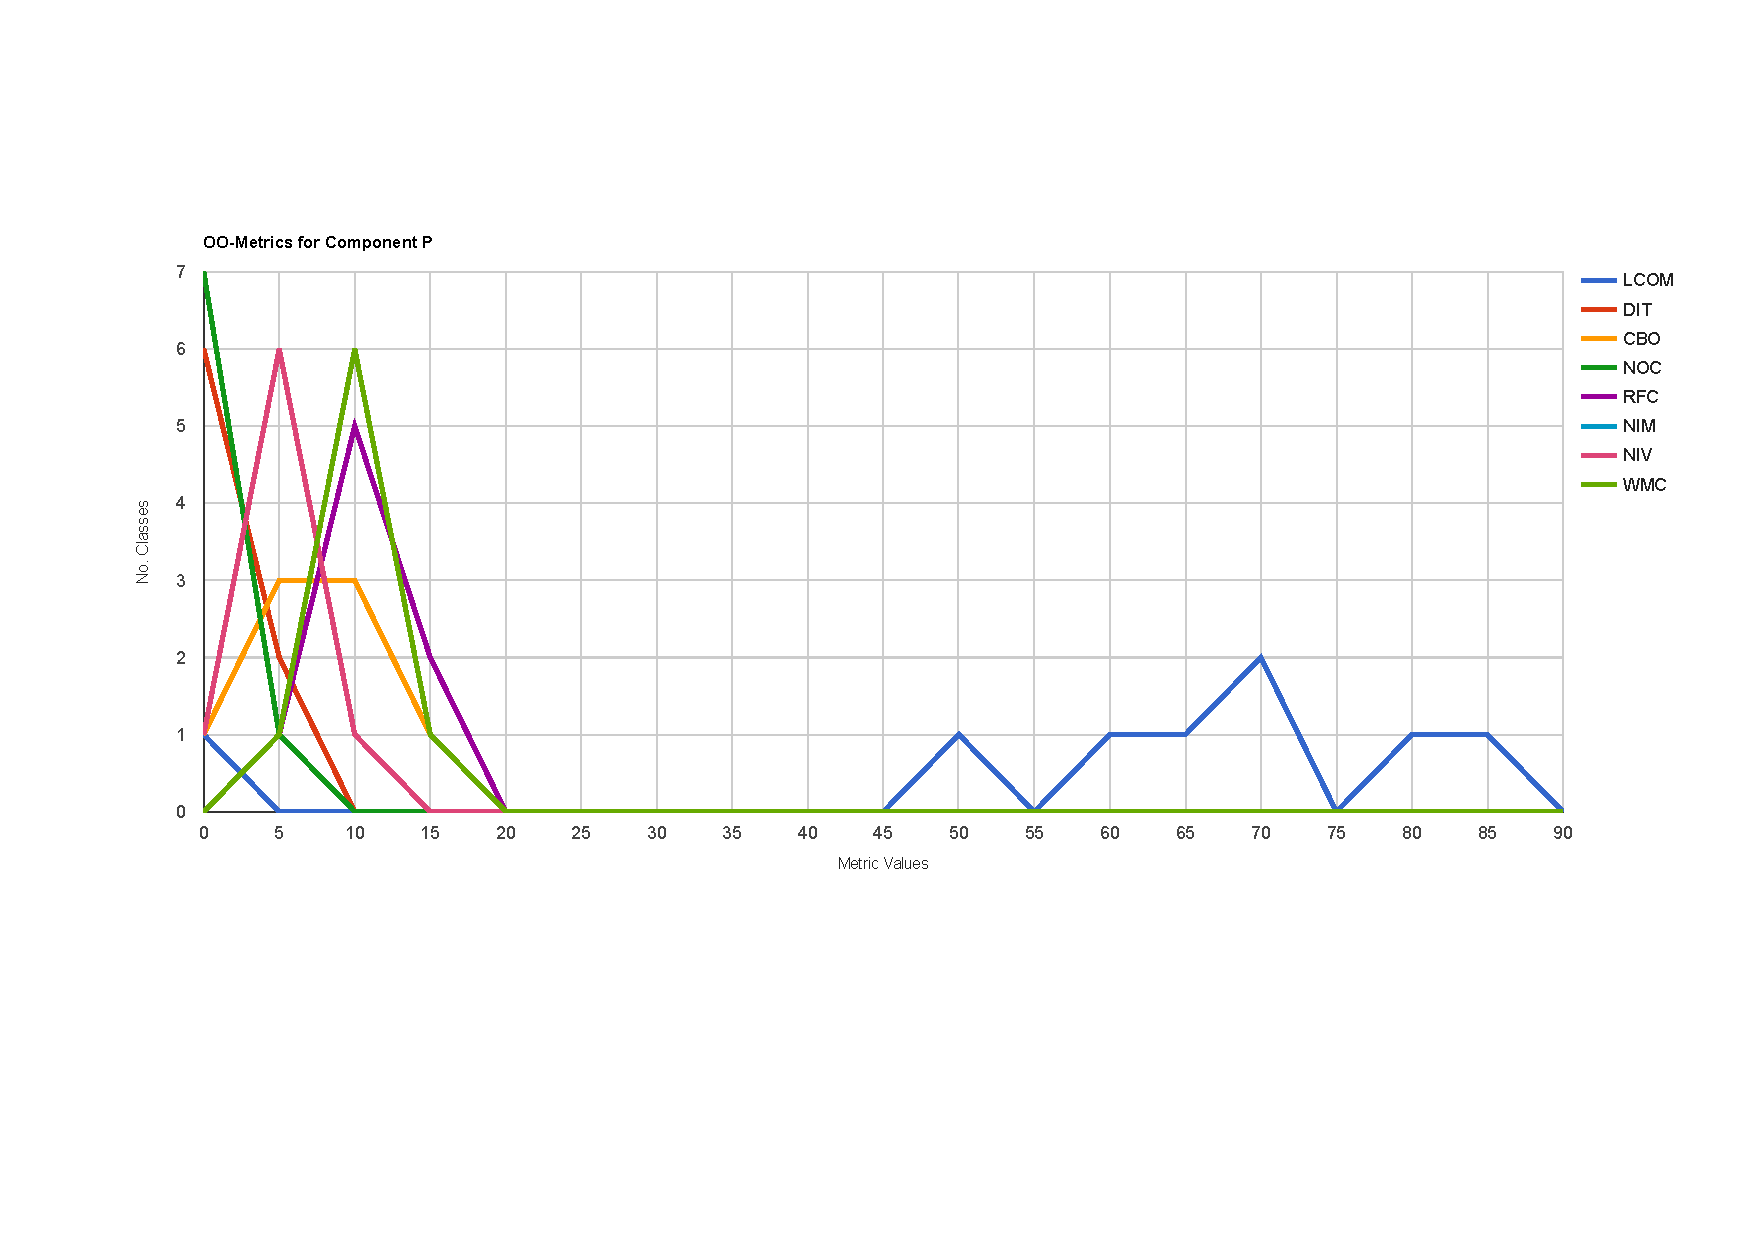
\includegraphics[width=\textwidth]{images/process.pdf}
	\end{figure}
\end{landscape}



\subsubsection{Component S}
Table \ref{tab:oometrics-sys} presents the descriptive statistics for Component S. Component S contains 4 files, which consists of 223 lines of code and 2 classes. The LCOM values show that there are possibilities to improve the design of this component by splitting up methods that does not share fields with each other to separate classes. Moreover, the results points out that none of the classes has any subclasses. However, the results reveal that one of the classes inherits methods and variables from a superclass. Moreover, WMC2 metric values indicate that classes have less complexity and greater polymorphism.

\begin{table}[]
\centering
\caption{OO-metrics for Component S}
\label{tab:oometrics-sys}
\begin{tabular}{|l|l|l|l|l|l|}
\hline
\textbf{Metric} & \textbf{Min} & \textbf{Max} & \textbf{Median} & \textbf{Sample Mean} & \textbf{Standard Deviation} \\ \hline
LCOM            & 33           & 50           & 41.5            & 41.5                 & 12.021                      \\ \hline
DIT             & 0            & 1            & 0.5             & 0.5                  & 0.707                       \\ \hline
CBO             & 3            & 6            & 4.5             & 4.5                  & 2.121                       \\ \hline
NOC             & 0            & 0            & 0               & 0                    & 0                           \\ \hline
RFC             & 6            & 9            & 7.5             & 7.5                  & 2.121                       \\ \hline
WMC             & 6            & 9            & 7.5             & 7.5                  & 2.121                       \\ \hline
WMC2            & 6           & 19            & 12.5            & 12.5                 & 9.192                         \\ \hline
NIM             & 6            & 9            & 7.5             & 7.5                  & 2.121                       \\ \hline
NIV             & 1            & 1            & 1               & 1                    & 0                           \\ \hline
\end{tabular}
\end{table}

 





\subsubsection{Component W}
Component W contains only one file. This file consists of 69 lines of code. In this component, we identified one class. This class has a LCOM value of 58, indicating low cohesion. The methods in this class do not share fields with each other, and the class should be split into separate classes. Moreover, DIT and NOC values of 0 indicates that this class does not inherit from a superclass, or has any subclasses. The results reports a CBO value of 4, implying that this class is not tightly coupled. WMC2 value of this class is set to 8, which implies that this class is not complex.





% Our results show that (whats good and wrong with these metrics, what can be done). 


% HVA SLAGS METRIKKER ER INTERESSANT, GÅ DYPERE INN PÅ DEM. F.EKS METHODS IN CLASS, HVA SIER DET OSS

% TOO MANY LINES OF CODE? CHECK SINGLE RESPONSBILITY PRINCIPLE, it states that every class or module should have responsbility for a single part of the funcitnaility provided by the software.'























\section{Identifying Code Smells using Automatic Approaches}
\label{sub:code_smell_detection}
As we explained in Chapter 2, one of the ways to identify design debt is to look at the number of code smells in the source code. Table \ref{tab:identifiedCodeSmell} describes the number of code smells that were identified using automatic.

\begin{table}[]
\centering
\caption{Number of Code Smells detected}
\label{tab:identifiedCodeSmell}
\begin{tabular}{|l|l|}
\hline
\textbf{Code Smell}                           & \textbf{Detected}    \\ \hline
Long Method                                   & 10          \\ \hline
Large Class                                   & 8          \\ \hline
Long Parameter List                           & 15          \\ \hline
%Data Clumps                                   & Bloaters          \\ \hline
%Switch Statements                             & O-O Abusers       \\ \hline
%Temporary Field                               & O-O Abusers       \\ \hline
%Refused Bequest                               & O-O Abusers       \\ \hline
%Alternative Classes with Different Interfaces & O-O Abusers       \\ \hline
%Parallel Inheritance Hierarchies              & O-O Abusers       \\ \hline
%Divergent Change                              & Change Preventers \\ \hline
%Shotgun Surgery                               & Change Preventers \\ \hline
%Lazy Class                                    & Dispensables      \\ \hline
%Data Class                                    & Dispensables      \\ \hline
Duplicated Code                               & Approximately 5\% of the source code. 39 files affected.       \\ \hline
Speculative Generality                        & 1153      \\ \hline
Dead Code 									  & 151 \\ \hline
\end{tabular}
\end{table}

\subsubsection{Duplicated Code}
Duplicated code is found by looking for pieces of code that appears at multiple places in the source code, both internally in a file or in another file. A piece of code is considered duplicated if the piece of code contains at least 10 lines of code and occurs at multiple places in the source code. Table \ref{tab:identifiedCodeSmell} reports the number of duplicated code found by SonarQube, expressed as a percentage value. Including the test files, the results show that roughly 5\% of the source code contains duplicated code. This corresponds to 4395 lines of code affecting 39 files across the system. By examining the results, we identified that roughly 54\% of the duplicated code is located in Component A. The other duplicated lines are spread across Component B, N, P, C, D, L, Ex, S, and G. Table \ref summarizes duplication in the different components, where "information" column summarizes number of files affected by duplicated code and the number of duplicated lines among these files.

\begin{table}[]
\centering
\caption{Duplication in Project Firmus}
\label{tab:duplicatedLines}
\begin{tabular}{|l|l|}
\hline
\textbf{Component}			& \textbf{Information} \\ \hline
Component A 				& 12 files, 2400 LOC \\ \hline
Component B 				& 6 files, 366 LOC \\ \hline
Component C 				& 3 files, 284 LOC \\ \hline
Component D 				& 2 files, 80 LOC \\ \hline
Component Ex 				& 4 files, 305 LOC \\ \hline
Component G 				& 4 files, 311 LOC \\ \hline
Component L 				& 1 file, 30 LOC \\ \hline
Component N 				& 3 files, 301 LOC \\ \hline
Component P 				& 2 files, 124 LOC \\ \hline
Component S 				& 2 files, 194 LOC \\ \hline
\end{tabular}
\end{table}


\subsubsection{Long Method}
Understand considers a Long Method as code smell if lines of code in method exceeds 200 lines. Using Understand, we identified 10 long methods, spread across six different files. 7 of 10 long methods are located in test files. 


\subsubsection{Long Parameter List}
Long Parameter List code smell is detected by comparing the total number of parameters in a method against a fixed threshold. The maximum number of parameters allowed in a method using CppDepend is set to 5. This means that 6 or more parameters in a method are considered as code smell. The results from CppDepend reports 15 hits of Long Parameter List code smell, where 3 hits are considered as critical. A Long Parameter List hit is critical when total of parameters in a method is higher than 8. The largest number of parameters in a method we identified was 12. These results were verified manually by examining the class diagrams for the corresponding methods.

\subsubsection{Speculative Generality}
Speculative Generality is detected by locating unused classes, methods, fields, or parameters. Table \ref{tab:speculativeGenerality} summarizes Speculative Generality code smell that were identified through a code analysis using Understand. The results are divided into the categories unused functions, unused local variables, and unused static globals. 

\begin{table}[]
\centering
\caption{Speculative Generality Results}
\label{tab:speculativeGenerality}
\begin{tabular}{|l|l|}
\hline
\textbf{Category}		& 	\textbf{Hits} \\ \hline
Unused Methods 			&	794  \\ \hline
Unused Local Variables 	& 	346	 \\ \hline
Unused Static Globals 	& 	13	 \\ \hline
\end{tabular}
\end{table}

%\subsubsection{Shotgun Surgery}
%The results shows that X classes are infected with the Shotgun Surgery code smell. 


\subsubsection{Dead Code}
Fowler and Beck\cite{1999:RID:311424} do not classify dead code as code smell. However, dead code should be classified as a code smell, as it is a quite common problem as it hinders code comprehension and makes the current program structure less obvious\cite{mantyla2003taxonomy}. We examined three types of "Dead Code" code smell in Project Firmus: "Commented Out" Code, Unreachable Code, and Unnecessary Includes in Header Files. In total, we found 151 hits of "Dead Code" code smell, which we have summarized in Table \ref{tab:deadCode}.

\begin{table}[]
\centering
\caption{Dead Code Results}
\label{tab:deadCode}
\begin{tabular}{|l|l|}
\hline
\textbf{Category}		& 	\textbf{Hits} \\ \hline
"Commented Out" Code 			&	67  \\ \hline
Unreachable Code 	& 	10	 \\ \hline
Unnecessary Includes in Header Files 	& 	74	 \\ \hline
\end{tabular}
\end{table}


\subsubsection{Large Class}
We were not able to identify any large classes using automatic tool. However, by counting the number of instances, variables, and methods using object-oriented metrics, we were able to identify some large classes in the system. Table X summarizes Large Class code smells. 

\subsubsection{God Classes}
CBO and LCOM can be useful to detect God Classes with support of LOC and WMC. (article: on the effectiveness of concern metrics to detect code smells: an empirical study)

A class with large values of WMC and RFC indicates many possible reponses since the class may have a large number of methods that can be executed. These values along with LCOM can be used to measure God Class code smell. By identiying 

5 files
%AL: LogicsEngine
%Autrologic: LogicsUnitDetectionZone
%Autrologic: Logicsunit
%AL: LogicsUnitFad (kasnkje)
%BLC: AclibTranslator



% ANtiåpattern, move down to metrics, point out that possible god classes may be antipatterns.



%How did we study the different code smells, the apporach and the results.
%The results from Table XX

%As we see, there are many code smells detected. We take a closer look at some of the classes; presented in UML diagrams here:




































